%%%%%%%%%%%%%%%%%%%%%%%%%%%%%%%%%%%%%%%%%%%%%%%%%%%%%%%%%%%%%%%%%%%%%%%%%%%%%%%%%%%%%%%%%%%%%%%%%%%%%%%%%%%%%%%%%%%%
%%% LaTeX Template para el Acoustic Congress 2020, que forma parte del XI Congreso Ibérico da Acústica,
%%% 51º Congreso Español de Acústica y TecniAcústica 2020
%%% Release 08/06/2020
%%% Desarrollado por Prof. William D'Andrea Fonseca de Ingeniería Acústica, UFSM, Brasil
%%% will.fonseca@eac.ufsm.br
%%%%%%%%%%%%%%%%%%%%%%%%%%%%%%%%%%%%%%%%%%%%%%%%%%%%%%%%%%%%%%%%%%%%%%%%%%%%%%%%%%%%%%%%%%%%%%%%%%%%%%%%%%%%%%%%%%%%
\documentclass[11pt, a4paper, twoside]{article}
%%%%%%%%%%%%%%%%%%%%%%%%%%%%%%%%%%%%%%%%%%%%%%%%%%%%
%%% Idioma y entrada
\usepackage[utf8]{inputenc} 
%%%%%%%%%%%%%%%%%%%%%%%%%%%%%%%%%%%%%%%%%%%%%%%%%%%%
\usepackage{ac2020}  %%% Configuración básica de plantilla
%%%%%%%%%%%%%%%%%%%%%%%%%%%%%%%%%%%%%%%%%%%%%%%%%%%%%%%%%%%%%%%%%%%%%%%%%%%%%%%%%%%%%%%%%%%%%%%%%%%%%%%%%%%%%%%%%%%%
%%% Datos del artículo

\Autores{Primer A. Autor, Segundo B. Autor, Tercer C. Autor} 
\AutoresAfiliaciones{Primer A. Autor$^1$, Segundo B. Autor$^1$, Tercer C. Autor$^2$} % Usa números como marcadores

%% Busque usar uma linha ou duas no máximo para cada autor
\Afiliaciones{$^1$\,Afiliación\\ \{e-mail del primer autor, e-mail del segundo autor\} \\[3pt]
$^2$\,Afiliación\\ \{e-mail del tercer autor\} }

\TituloCompleto{INSTRUCCIONES PARA LA PREPARACIÓN DE COMUNICACIONES\linebreak PARA EL “CONGRESO ACÚSTICA 2020”}

\PalavrasClave{instrucciones, formato, reglas, recomendaciones, no usar más de 5 palabras}
\Keywords{instructions, format, rules, recommendations, maximum of 5}

\PACS{xx.xx.Nn, xx.xx.Nn}

\Resumen{El resumen deberá consistir en uno o dos párrafos, de 6 a 10 líneas. El asunto deberá ser presentando con claridad y objetividad incluyendo los resultados principales y las conclusiones del trabajo. Este deberá restringirse a la primera página de la comunicación.}

\Abstract{An abstract in English should also be included. The abstract should consist of one or two paragraphs, with a total of 6 to 10 lines, clearly stating the objectives, main results and conclusions of the work. The abstract should not continue to the second page.}

%%%%%%%%%%%%%%%%%%%%%%%%%%%%%%%%%%%%%%%%%%%%%%%%%%%%%%%%%%%%%%%%%%%%%%%%%%%%%%%%%%%%%%%%%%%%%%%%%%%%%%%%%%%%%%%%%%%%
%%%%%%%%%%%%%%%%%%%%%%%%%%%%%%%%%%%%%%%%%%%%%%%%%%%%%%%%%%%%%%%%%%%%%%%%%%%%%%%%%%%%%%%%%%%%%%%%%%%%%%%%%%%%%%%%%%%%
\begin{document} \setcounter{page}{1}
%%%%%%%%%%%%%%%%%%%%%%%%%%%%%%%%%%%%%%%%%%%%%%%%%%%%%%%%%%%%%%%%%%%%%%%%%%%%%%%%%%%%%%%%%%%%%%%%%%%%%%%%%%%%%%%%%%%%
%%%%%%%%%%%%%%%%%%%%%%%%%%%%%%%%%%%%%%%%%%%%%%%%%%%%%%%%%%%%%%%%%%%%%%%%%%%%%%%%%%%%%%%%%%%%%%%%%%%%%%%%%%%%%%%%%%%%
%%% Template para de LaTeX para o evento 12º Congresso Iberoamericano de Acústica 
%%%                      em conjunto com XXIX Encontro da Sobrac
%%% Baseado no modelo da Revista Acústica e Vibrações da Sobrac
%%% Release 19/04/2022
%%%	Desenvolvido por por Prof. William D'Andrea Fonseca, Dr. Eng. - Engenharia Acústica UFSM
%%% will.fonseca@eac.ufsm.br
%%%%%%%%%%%%%%%%%%%%%%%%%%%%%%%%%%%%%%%%%%%%%%%%%%%%%%%%%%%%%%%%%%%%%%%%%%%%%%%%%%%%%%%%%%%%%%%%%%%%%%%%%%%%%%%%%%%%
%%%%%%%%%%%%%%%%%%%%%%%%%%%%%%%%%%%%%%%%%%%%%%%%%%%%%%%%%%%%%%%%%%%%%%%%%%%%%%%%%%%%%%%%%%%%%%%%%%%%%%%%%%%%%%%%%%%%
%% Estilo do artigo
\pagestyle{plain}
%%%%%%%%%%%%%%%%%%%%%%%%%%%%%%%%%%%%%%%%%%%%%%%%%%%%%%%%%%%%%%%%%%%%%%%%%%%%%%%%%%%%%%%%%%%%%%%%%%%%%%%%%%%%%%%%%%%%
%%% Primeira página
\thispagestyle{firststyle}
% \newgeometry{top=2.1cm, bottom=2cm, left=1.9cm, right=1.9cm, headsep=5mm}
%%%%%%%%%%%%%%%%%%%%%%%%%%%%%%%%%%%%%%%%%%%%%%%%%%%%%%%%%%%%%%%%%%%%%%%%%%%%%%%%%%%%%%%%%%%%%%%%%%%%%%%%%%%%%%%%%%%%
\begin{textblock}{200}(150.2,283.51)
\fontsize{8}{8}\selectfont\sffamily 
DOI:~\href{https://doi.org/\DOIArtigo}{\DOIArtigo}
\end{textblock}
%%% Título
\begin{textblock}{170}(37,12)
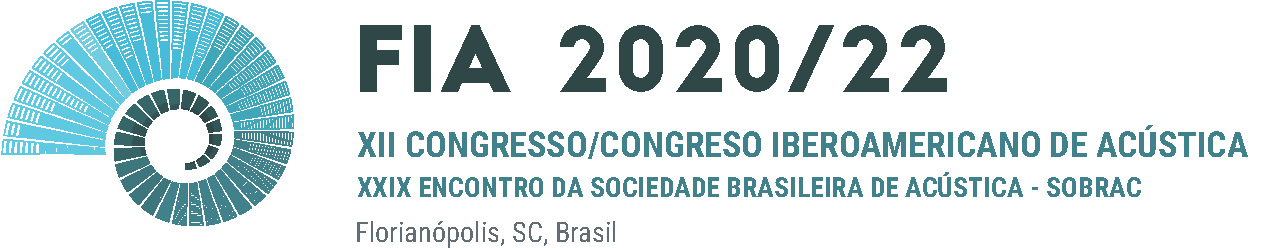
\includegraphics[width=0.82\textwidth,page=1]{FIA-logo.pdf}
\end{textblock}

\twocolumn[
\begin{@twocolumnfalse}
\vspace{60pt}
\begin{center}
{\fontsize{18}{22}\selectfont\bfseries 
%% Título
%%%%%%%%%%%%%%%%%%%%%%%%%%%%%%%%%%%%%%%%%%%%%%%%%%%%%%%%%%%%%%%%%%%%%%%%%%%%%%%%%%%%%%%%%%%%%%%%%%%%%%%%%%%%%%%%%%%%
\TituloCompletoArtigo \bookmark[page=1,level=1]{Título e Resumo}
%%%%%%%%%%%%%%%%%%%%%%%%%%%%%%%%%%%%%%%%%%%%%%%%%%%%%%%%%%%%%%%%%%%%%%%%%%%%%%%%%%%%%%%%%%%%%%%%%%%%%%%%%%%%%%%%%%%%
\par}

%%%%%%%%%%%%%%%%%%%%%%%%%%%%%%%%%%%%%%%%%%%%%%%%%%%%%%%%%%%%%%%%%%%%%%%%%%%%%%%%%%%%%%%%%%%%%%%%%%%%%%%%%%%%%%%%%%%
%%%%%%%%%%%%%%%%%%%%%%%%%%%%%%%%%%%%%%%%%%%%%%%%%%%%%%%%%%%%%%%%%%%%%%%%%%%%%%%%%%%%%%%%%%%%%%%%%%%%%%%%%%%%%%%%%%%
\vspace{12pt}
{\fontsize{11}{13}\selectfont \bfseries 
%% Autores
%%%%%%%%%%%%%%%%%%%%%%%%%%%%%%%%%%%%%%%%%%%%%%%%%%%%%%%%%%%%%%%%%%%%%%%%%%%%%%%%%%%%%%%%%%%%%%%%%%%%%%%%%%%%%%%%%%%
\AutoresFiliacoesArtigo
%%%%%%%%%%%%%%%%%%%%%%%%%%%%%%%%%%%%%%%%%%%%%%%%%%%%%%%%%%%%%%%%%%%%%%%%%%%%%%%%%%%%%%%%%%%%%%%%%%%%%%%%%%%%%%%%%%%
\par}

\vspace{2mm}
{\fontsize{9}{11}\selectfont 
%% Filiações
%%%%%%%%%%%%%%%%%%%%%%%%%%%%%%%%%%%%%%%%%%%%%%%%%%%%%%%%%%%%%%%%%%%%%%%%%%%%%%%%%%%%%%%%%%%%%%%%%%%%%%%%%%%%%%%%%%%
\FiliacoesArtigo
%%%%%%%%%%%%%%%%%%%%%%%%%%%%%%%%%%%%%%%%%%%%%%%%%%%%%%%%%%%%%%%%%%%%%%%%%%%%%%%%%%%%%%%%%%%%%%%%%%%%%%%%%%%%%%%%%%%%
\par}
\end{center}

\vspace{-5mm}{\color{FIABlue}\rule{\textwidth}{0.4pt}}
%%%%%%%%%%%%%%%%%%%%%%%%%%%%%%%%%%%%%%%%%%%%%%%%%%%%%%%%%%%%%%%%%%%%%%%%%%%%%%%%%%%%%%%%%%%%%%%%%%%%%%%%%%%%%%%%%%%%
%%%%%%%%%%%%%%%%%%%%%%%%%%%%%%%%%%%%%%%%%%%%%%%%%%%%%%%%%%%%%%%%%%%%%%%%%%%%%%%%%%%%%%%%%%%%%%%%%%%%%%%%%%%%%%%%%%%%
%%% Resumo e palavras-chave
\ResumoTexto
%%%%%%%%%%%%%%%%%%%%%%%%%%%%%%%%%%%%%%%%%%%%%%%%%%%%%%%%%%%%%
%%% Title, abstract and keywords
%%%%%%%%%%%%%%%%%%%%%%%%%%%%%%%%%%%%%%%%%%%%%%%%%%%%%%%%%%%%%
%%% Title
\begin{otherlanguage*}{english}
{\EnglishTitle}
%%%%%%%%%%%%%%%%%%%%%%%%%%%%%%%%%%%%%%%%%%%%%%%%%%%%%%%%%%%%%%%%%%%%%%%%%%%%%%%%%%%%%%%%%%%%%%%%%%%%%%%%%%%%%%%%%%%%
%%%%%%%%%%%%%%%%%%%%%%%%%%%%%%%%%%%%%%%%%%%%%%%%%%%%%%%%%%%%%%%%%%%%%%%%%%%%%%%%%%%%%%%%%%%%%%%%%%%%%%%%%%%%%%%%%%%%
%%% Abstract
		{\textbf{Abstract}} \vspace{5pt}
		
		{\fontsize{11}{12.5}\selectfont
		\AbstractArtigo
		\par}
		%%%%%%%%%%%%%%%%%%%%%%%%% Keywords
		\vspace{0.7\baselineskip} \fontsize{11}{12}\selectfont
		\textbf{Keywords: }{\fontsize{11}{12}\selectfont 
		\KeywordsArtigo.
		\par}
		%%%%%%%%%%%%%%%%%%%%%%%%% PACs:
		\PACSEnglish
	  \vspace{6mm}
\end{otherlanguage*}		
%%%%%%%%%%%%%%%%%%%%%%%%%%%%%%%%%%%%%%%%%%%%%%%%%%%%%%%%%%%%%%%%%%%%%%%%%%%%%%%%%%%%%%%%%%%%%%%%%%%%%%%%%%%%%%%%%%%%
%%%%%%%%%%%%%%%%%%%%%%%%%%%%%%%%%%%%%%%%%%%%%%%%%%%%%%%%%%%%%%%%%%%%%%%%%%%%%%%%%%%%%%%%%%%%%%%%%%%%%%%%%%%%%%%%%%%%
\end{@twocolumnfalse}
]
% \restoregeometry 
% \newgeometry{top=2.1cm, bottom=2cm, left=1.9cm, right=1.9cm, headsep=5mm}
\pagestyle{plain}

%%%%%%%%%%%%%%%%%%%%%%%%%%%%%%%%%%%%%%%%%%%%%%%%%%%%%%%%%%%%%%%%%%%%%%%%%%%%%%%%%%%%%%%%%%%%%%%%%%%%%%%%%%%%%%%%%%%%
% EOF

%%%%%%%%%%%%%%%%%%%%%%%%%%%%%%%%%%%%%%%%%%%%%%%%%%%%%%%%%%%%%%%%%%%%%%%%%%%%%%%%%%%%%%%%%%%%%%%%%%%%%%%%%%%%%%%%%%%%
%%%%%%%%%%%%%%%%%%%%%%%%%%%%%%%%%%%%%%%%%%%%%%%%%%%%%%%%%%%%%%%%%%%%%%%%%%%%%%%%%%%%%%%%%%%%%%%%%%%%%%%%%%%%%%%%%%%%
%%% Artículo
%%%%%%%%%%%%%%%%%%%%%%%%%%%%%%%%%%%%%%%%%%%%%%%%%%%%%%%%%%%%%%%%%%%%%%%%%%%%%%%%%%%%%%%%%%%%%%%%%%%%%%%%%%%%%%%%%%%%
%%%%%%%%%%%%%%%%%%%%%%%%%%%%%%%%%%%%%%%%%%%%%%%%%%%%%%%%%%%%%%%%%%%%%%%%%%%%%%%%%%%%%%%%%%%%%%%%%%%%%%%%%%%%%%%%%%%%
\section{Introducción}

Este documento constituye el template/modelo a seguir para la preparación de los artículos para el Congreso Acústica 2020. Es necesario incluir las referencias PACS (Physics and Astronomy Classification Scheme) sobre los temas a los que se refiere el artículo. El listado completo de estas referencias se puede obtener en website de SEA (\url{http://www.sea-acustica.es/?id=46}).


%%%%%%%%%%%%%%%%%%%%%%%%%%%%%%%%%%%%%%%%%%%%%%%%%%%%%%%%%%%%%%%%%%%%%%%%%%%%%%%%%%%%%%%%%%%%%%%%%%%%%%%%%%%%%%%%%%%%
%%%%%%%%%%%%%%%%%%%%%%%%%%%%%%%%%%%%%%%%%%%%%%%%%%%%%%%%%%%%%%%%%%%%%%%%%%%%%%%%%%%%%%%%%%%%%%%%%%%%%%%%%%%%%%%%%%%%
\section{Presentación y publicación}

En esta sección, se presentan los detalles para la presentación y publicación.

%%%%%%%%%%%%%%%%%%%%%%%%%%%%%%%%%%%%%%%%%%%%%%%%%%%%%%%%%%%%%%%%%%%%%%%%%%%%%%%%%%%%%%%%%%%%%%%%%%%%%%%%
\subsection{Presentación de las comunicaciones}

Las comunicaciones deberán ser presentadas en formato electrónico PDF, a través de la página del Congreso \url{http://www.spacustica.pt/acustica2020/index.html}.

\clearpage
%%%%%%%%%%%%%%%%%%%%%%%%%%%%%%%%%%%%%%%%%%%%%%%%%%%%%%%%%%%%%%%%%%%%%%%%%%%%%%%%%%%%%%%%%%%%%%%%%%%%%%%%%%%%%%%%%%%%
%%%%%%%%%%%%%%%%%%%%%%%%%%%%%%%%%%%%%%%%%%%%%%%%%%%%%%%%%%%%%%%%%%%%%%%%%%%%%%%%%%%%%%%%%%%%%%%%%%%%%%%%%%%%%%%%%%%%
\section{Reglas generales de redacción}

La redacción de los artículos debe ser como se muestra en el template/modelo presentado en este documento. La comunicación no deberá exceder a 12 páginas de tamaño A4 y el fichero no deberá exceder de 5~MB.


%%%%%%%%%%%%%%%%%%%%%%%%%%%%%%%%%%%%%%%%%%%%%%%%%%%%%%%%%%%%%%%%%%%%%%%%%%%%%%%%%%%%%%%%%%%%%%%%%%%%%%%%
\subsection{Redacción del texto}

En esta sección, se presentan los detalles de formato.


%%%%%%%%%%%%%%%%%%%%%%%%%%%%%%%%%%%%%%%%%%%%%%%%%%%%%%%%%%%%%%%%%%%%%%%%%%%%%%%%%%%%%%%%%%%%%%%%%%%%%%%%
\subsubsection{Tablas y figuras}

Las tablas y figuras deberán estar centradas y numeradas de forma consecutiva, con una leyenda descriptiva centrada en la página (ver ejemplo de \tabla{tab.exemplo} y \Figura{fig:beamforming}).


\begin{table}[H]
  \centering 
  \caption{Ejemplo de tabla xxx / yyy.}
	\fontsize{11}{12}\selectfont 
    \begin{tabular}{C{2.8cm} | C{2.8cm}}
    \toprule
		\SetRowColor{LightOrange}
    \textbf{ xxx } & \textbf{yyy} \\
	  \midrule
		10 & 3120\\
		\rowcolor[gray]{.95} 40	& 2555\\
		50 & 1100\\
    \bottomrule
    \end{tabular}
    \label{tab.exemplo}%
\end{table}%


\begin{figure}[H]
	\centering
	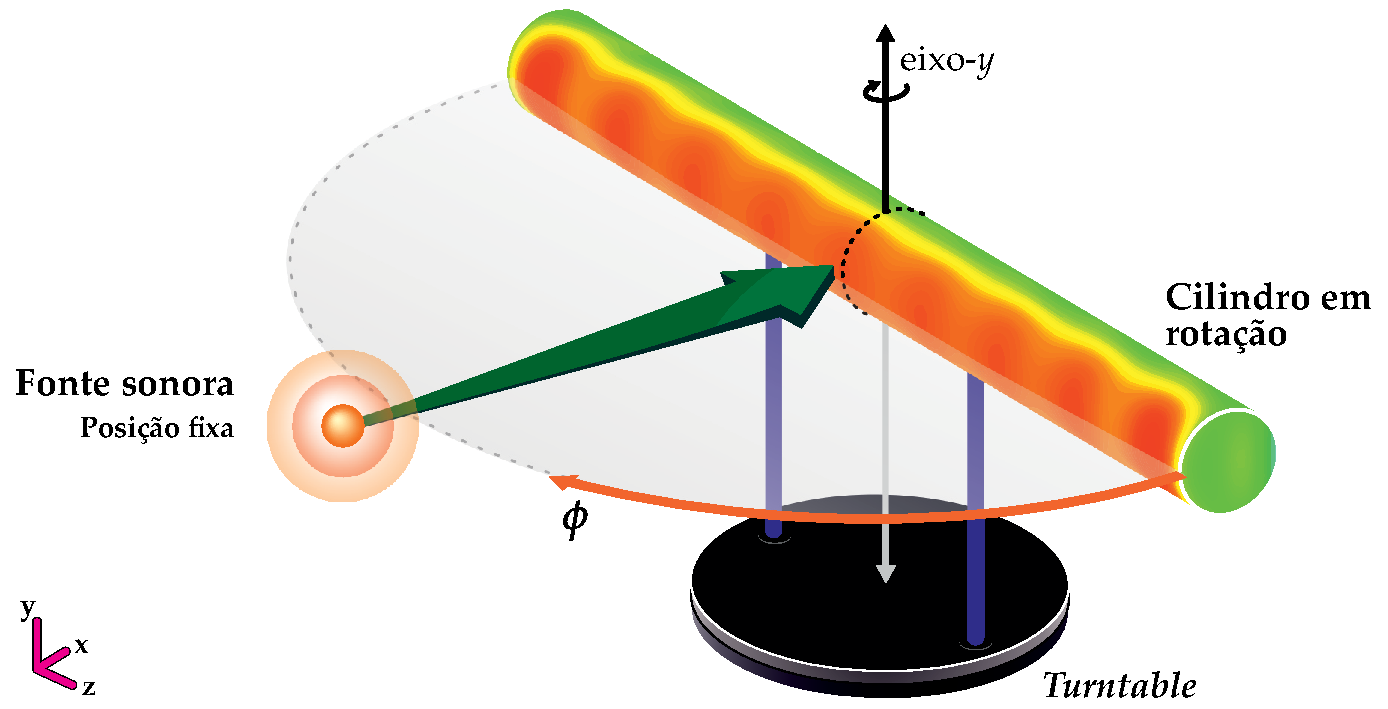
\includegraphics[width=0.75\linewidth]{Figuras/Measurement-Scheme-Fonseca-2013.pdf}%
	\caption{Ejemplo de figura con leyenda (adaptado de \cite{Fonseca-2013}).}%
	\label{fig:beamforming}%
\end{figure}


%%%%%%%%%%%%%%%%%%%%%%%%%%%%%%%%%%%%%%%%%%%%%%%%%%%%%%%%%%%%%%%%%%%%%%%%%%%%%%%%%%%%%%%%%%%%%%%%%%%%%%%%
\subsubsection{Ecuaciones}

Las ecuaciones deberán estar numeradas secuencialmente utilizando caracteres árabes entre paréntesis. Las expresiones deberán estar centradas dejando espacios de 6 por encima y por debajo para separarlas del resto del texto. A título de ejemplo 
%
\begin{equation}
Ax = b \,,
\label{eq:eq1}
\end{equation}
%
donde $A$ y $b$ son constantes. Deberán ser utilizados símbolos, convenciones y unidades SI.


%%%%%%%%%%%%%%%%%%%%%%%%%%%%%%%%%%%%%%%%%%%%%%%%%%%%%%%%%%%%%%%%%%%%%%%%%%%%%%%%%%%%%%%%%%%%%%%%%%%%%%%%
\subsection{Citas de referencias bibliográficas}

A lo largo del texto las referencias bibliográficas deberán ser citadas utilizando números entre paréntesis rectos \cite{Fonseca-2013,ref2,TADEU2006,ref4,refBranco,ref6,Brebbia}. En la sección de referencias, siempre que sea posible, incluya el ISBN, DOI (con enlace) y/o enlace con la dirección en línea en la que está disponible el documento mencionado.

%%%%%%%%%%%%%%%%%%%%%%%%%%%%%%%%%%%%%%%%%%%%%%%%%%%%%%%%%%%%%%%%%%%%%%%%%%%%%%%%%%%%%%%%%%%%%%%%%%%%%%%%%%%%%%%%%%%%%%%%%%%%%%%%%%%%%%%%%%%%%%%%%%%%%%%%%%%%%%%%%%%%%%%%%%%%%%%%%%%%%%%%%%
\section{Conclusiones}

Por lo menos uno de los autores deberá inscribirse y regularizar el correspondiente pago de la cuota de inscripción. Así su comunicación será aceptada para presentación en el Congreso y publicada en las respectivas Actas.

%%%%%%%%%%%%%%%%%%%%%%%%%%%%%%%%%%%%%%%%%%%%%%%%%%%%%%%%%%%%%%%%%%%%%%%%%%%%%%%%%%%%%%%%%%%%%%%%%%%%%%%%%%%%%%%%%%%%%%%%%%%%%%%%%%%%%%%%%%%%%%%%%%%%%%%%%%%%%%%%%%%%%%%%%%%%%%%%%%%%%%%%%%
\subsection*{Agradecimientos}

Los agradecimientos alusivos a personas o entidades deberán ser incluidos al final del texto, en epígrafe propio, antes de las referencias.

%%%%%%%%%%%%%%%%%%%%%%%%%%%%%%%%%%%%%%%%%%%%%%%%%%%%%%%%%%%%%%%%%%%%%%%%%%%%%%%%%%%%%%%%%%%%%%%%%%%%%%%%%%%%%%%%%%%%
%%%%%%%%%%%%%%%%%%%%%%%%%%%%%%%%%%%%%%%%%%%%%%%%%%%%%%%%%%%%%%%%%%%%%%%%%%%%%%%%%%%%%%%%%%%%%%%%%%%%%%%%%%%%%%%%%%%%
%%% Referências
\renewcommand{\refname}{Referencias} 
\bibliographystyle{unsrtnat2}
\bibliography{bibliografia}
%%%%%%%%%%%%%%%%%%%%%%%%%%%%%%%%%%%%%%%%%%%%%%%%%%%%%%%%%%%%%%%%%%%%%%%%%%%%%%%%%%%%%%%%%%%%%%%%%%%%%%%%
%%%%%%%%%%%%%%%%%%%%%%%%%%%%%%%%%%%%%%%%%%%%%%%%%%%%%%%%%%%%%%%%%%%%%%%%%%%%%%%%%%%%%%%%%%%%%%%%%%%%%%%%
\end{document}
% EOF %%%%%%%%%%%%%%%%%%%%%%%%%%%%%%%%%%%%%%%%%%%%%%%%%%%%%%%%%%%%%%%%%%%%%%%%%%%%%%%%%%%%%%%%%%%%%%%%%%